\documentclass[12pt,a4paper]{article}

% ── Packages ──────────────────────────────────────────────────────────────────
\usepackage[a4paper, margin=2.5cm]{geometry}
\usepackage{setspace}
\usepackage{fontenc}
\usepackage[utf8]{inputenc}
\usepackage{lmodern}
\usepackage{microtype}
\usepackage{parskip}
\usepackage{graphicx}
\usepackage{float}
\usepackage{hyperref}
\usepackage{xcolor}
\usepackage{listings}
\usepackage{tocloft}
\usepackage{caption}
\usepackage{booktabs}
\usepackage{enumitem}
\usepackage{amsmath}
\usepackage{fancyhdr}
\usepackage{titlesec}

% ── Spacing ───────────────────────────────────────────────────────────────────
\onehalfspacing

% ── Header / Footer ───────────────────────────────────────────────────────────
\pagestyle{fancy}
\fancyhf{}
\lhead{\small\textit{COMP47980: Generative AI And Language Models, Project Report, 2026}}
\rhead{\small\thepage}
\renewcommand{\headrulewidth}{0.4pt}

% ── Section title formatting ──────────────────────────────────────────────────
\titleformat{\section}{\large\bfseries}{}{0em}{\thesection.\quad}
\titleformat{\subsection}{\normalsize\bfseries}{}{0em}{\thesubsection\quad}

% ── Code listing style ────────────────────────────────────────────────────────
\definecolor{codebg}{gray}{0.96}
\definecolor{codeframe}{gray}{0.75}
\lstset{
  backgroundcolor=\color{codebg},
  frame=single,
  rulecolor=\color{codeframe},
  basicstyle=\ttfamily\small,
  breaklines=true,
  showstringspaces=false,
  language=Python,
  keywordstyle=\color{blue}\bfseries,
  commentstyle=\color{gray}\itshape,
  stringstyle=\color{teal},
  numbers=left,
  numberstyle=\tiny\color{gray},
  numbersep=8pt,
}

\lstdefinelanguage{json}{
  morestring=[b]",
  morecomment=[l]{//},
  literate=
    *{0}{{{\color{teal}0}}}{1}
     {1}{{{\color{teal}1}}}{1}
     {2}{{{\color{teal}2}}}{1}
     {3}{{{\color{teal}3}}}{1}
     {4}{{{\color{teal}4}}}{1}
     {5}{{{\color{teal}5}}}{1}
     {6}{{{\color{teal}6}}}{1}
     {7}{{{\color{teal}7}}}{1}
     {8}{{{\color{teal}8}}}{1}
     {9}{{{\color{teal}9}}}{1}
     {:}{{{\color{gray}{:}}}}{1}
     {,}{{{\color{gray}{,}}}}{1},
  stringstyle=\color{teal},
  commentstyle=\color{gray}\itshape,
}

% ── Hyperref setup ────────────────────────────────────────────────────────────
\hypersetup{
  colorlinks=true,
  linkcolor=blue!70!black,
  urlcolor=blue!70!black,
  citecolor=blue!70!black,
}

% ── ToC / LoF dot leaders ────────────────────────────────────────────────────
\renewcommand{\cftsecleader}{\cftdotfill{\cftdotsep}}

% ─────────────────────────────────────────────────────────────────────────────
\begin{document}

% ── Title Page ────────────────────────────────────────────────────────────────
\begin{titlepage}
  \centering
  \vspace*{1cm}
  {\small\textit{COMP47980: Generative AI And Language Models, Project Report, 2026}}
  \vspace{2cm}

  {\fontsize{32}{40}\selectfont\bfseries AI Tutor}\\[0.6em]
  {\Large An Adaptive Learning Assistant That Converts\\[0.3em]
   Passive Technical Content into Active Study Workflows}

  \vspace{2.5cm}

  {\large\bfseries Dat Tran}\\[0.3em]
  {\normalsize Student ID: [Your Student ID]}\\[0.5em]
  {\normalsize \href{mailto:dattran@example.com}{[your-email@ucd.ie]}}

  \vspace{2.5cm}

  \begin{center}
    \fbox{
      \parbox{0.8\textwidth}{\centering\vspace{1cm}
        \textit{AI Tutor: from lecture slides to mastery ---}\\[0.3em]
        \textit{one concept at a time.}
        \vspace{1cm}}
    }
  \end{center}

  \vfill
  {\normalsize May 2026}
\end{titlepage}

% ── Table of Contents ─────────────────────────────────────────────────────────
\newpage
\setcounter{page}{2}
\thispagestyle{plain}
{\large\bfseries Table of Contents}
\vspace{0.5em}
\tableofcontents

% ── List of Figures ───────────────────────────────────────────────────────────
\newpage
\thispagestyle{plain}
{\large\bfseries List of Figures}
\vspace{0.5em}
\listoffigures

% ─────────────────────────────────────────────────────────────────────────────
\newpage
\setcounter{page}{1}

% =============================================================================
\section{Introduction}
% =============================================================================

AI Tutor is an AI-powered study assistant that manages technical documents (lecture notes, PDF textbooks, scanned slides) into structured, and provides an interactive and adaptive learning workflows. Research in cognitive science consistently shows that active recall, the act of retrieving information from memory under test conditions, produces significantly better long-term retention than passive re-reading \cite{roediger2006test}. However, most students default to highlighting notes or re-reading slides, and existing tools such as ChatGPT, while capable of answering questions on demand, cannot track what a student has already studied, identify knowledge gaps and provide a personalised and adaptive learning experience. AI Tutor closes this gap by decomposing uploaded material into discrete concepts organised in a searchable topic hierarchy, then generating a personalised practice questions that target the student's weakest areas, grading answers and persisting session history across runs

% =============================================================================
\section{Assistant Design: A Schematic View}
% =============================================================================

\subsection{High-Level Architecture}

Figure~\ref{fig:architecture} shows the overall architecture of AI Tutor.
Every major subsystem is a class that either extends \texttt{Agent} (the
ReAct engine) or composes it.

\begin{figure}[H]
\centering
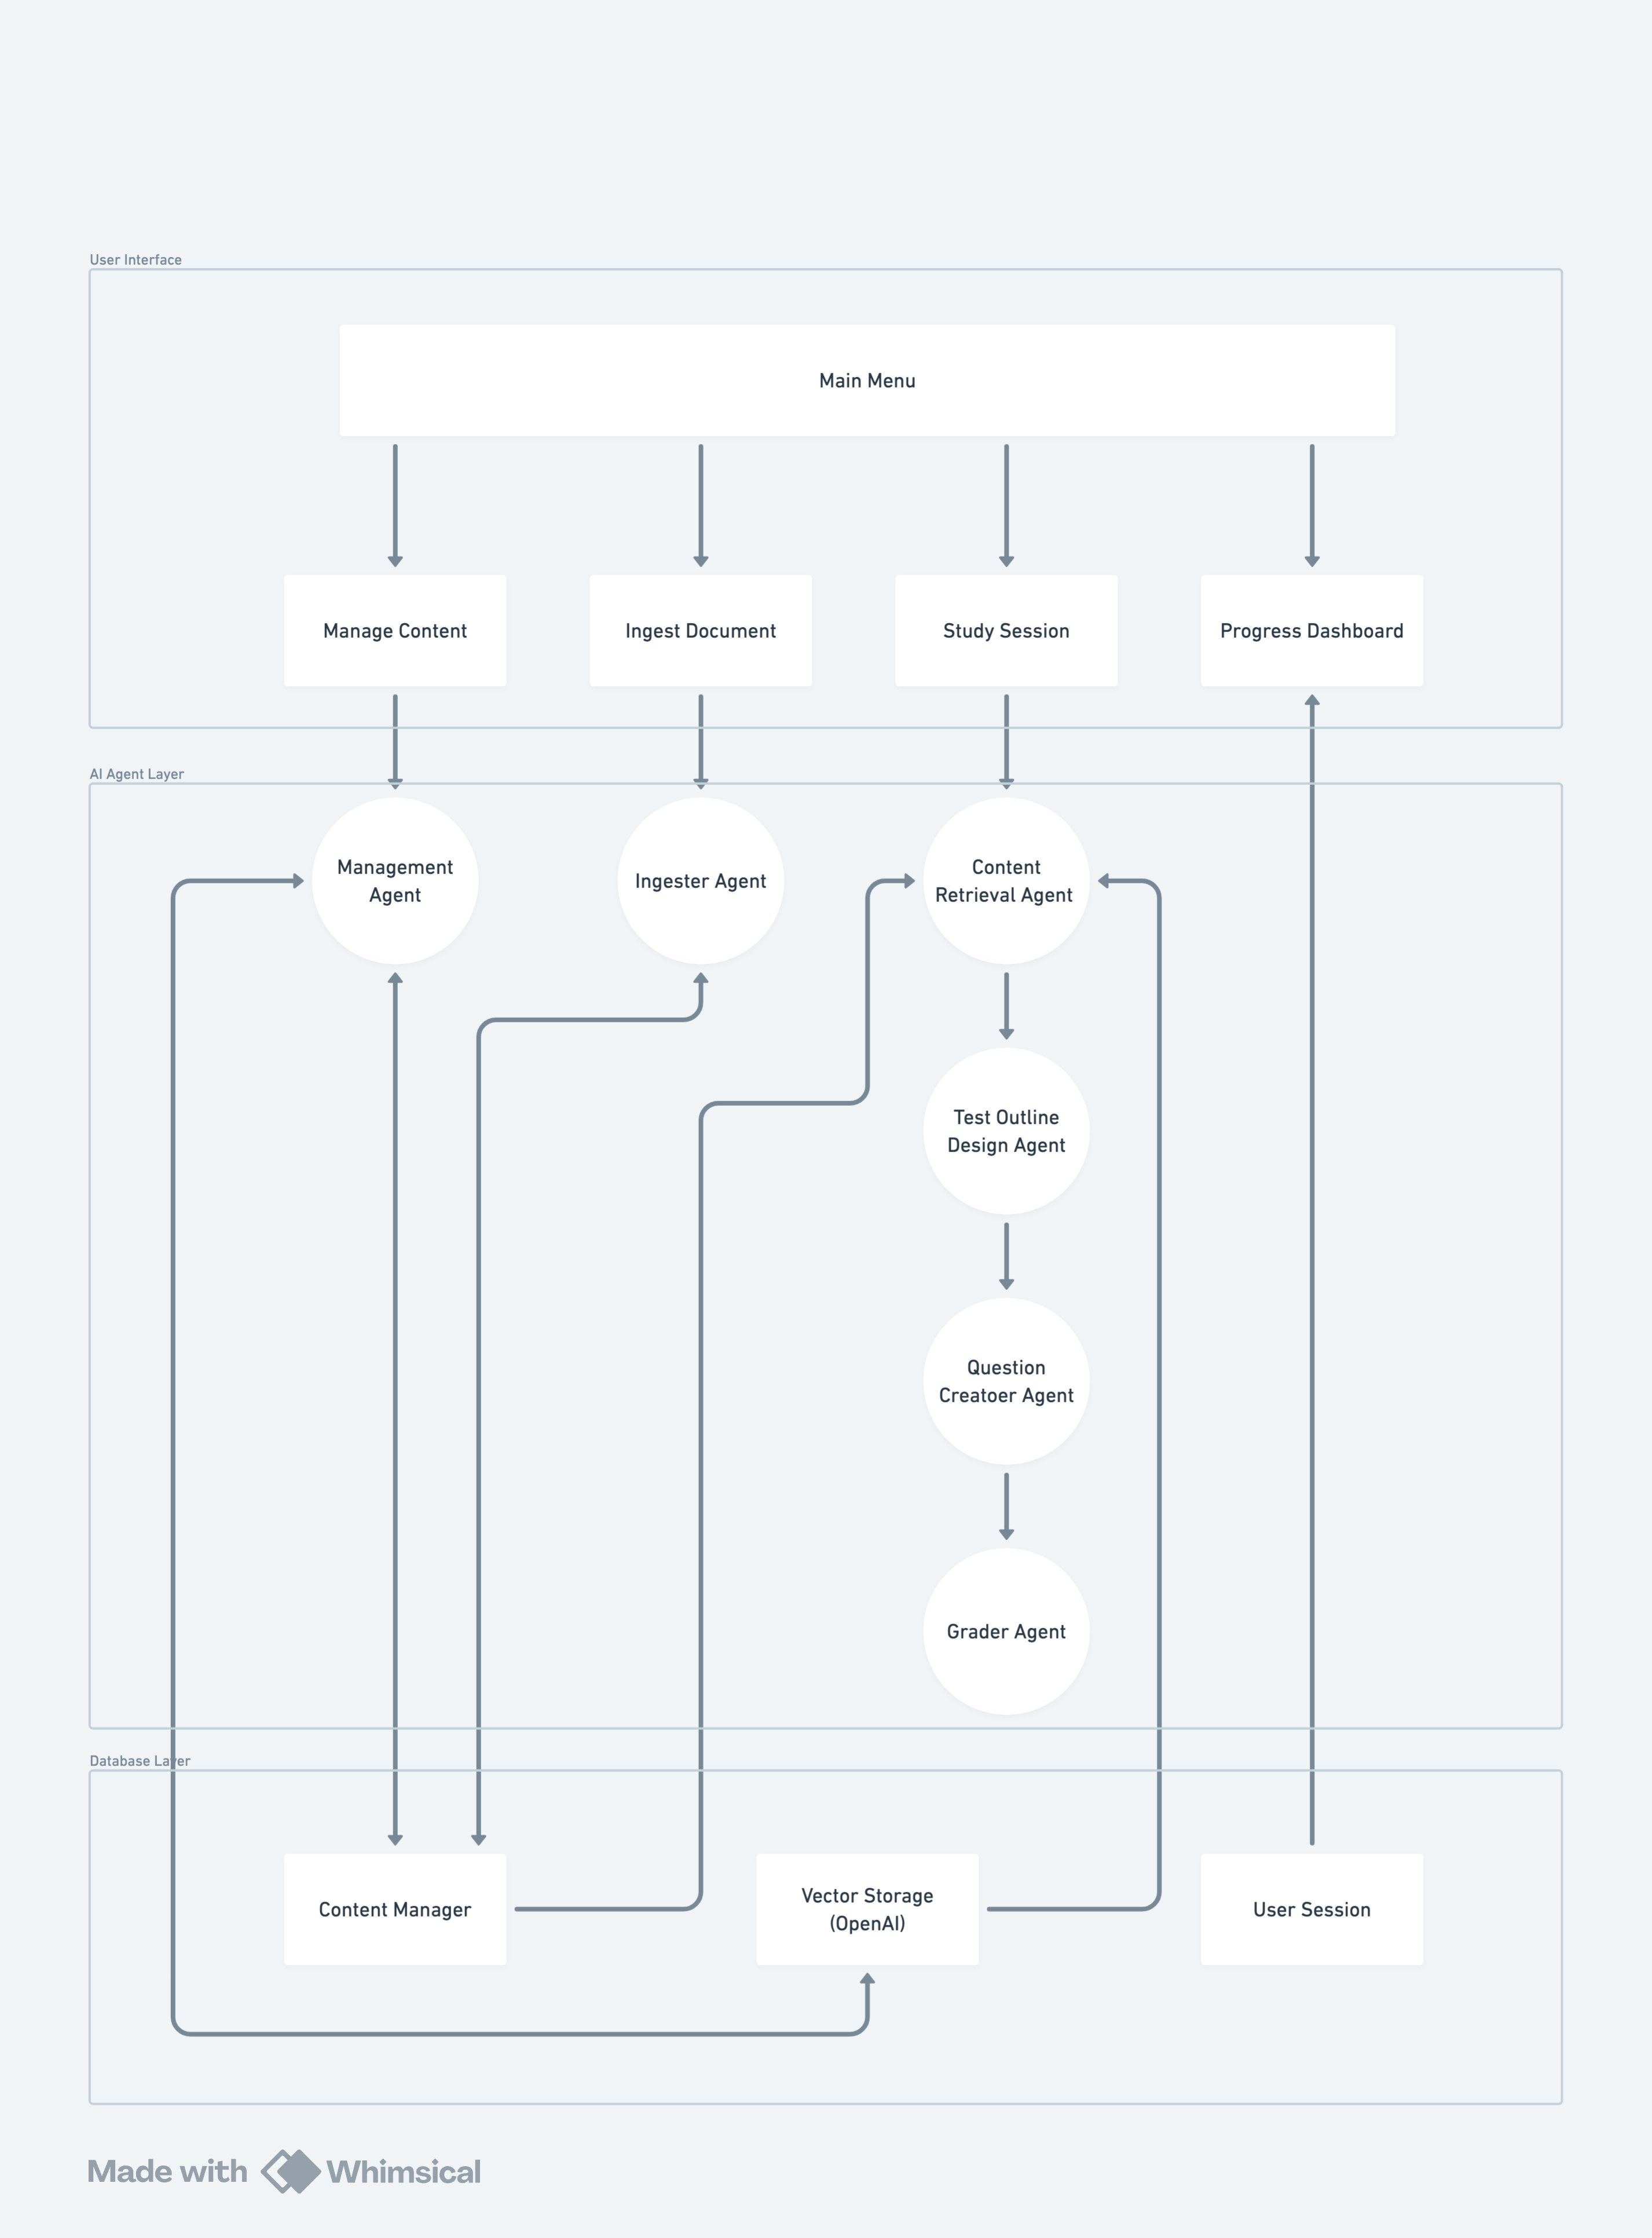
\includegraphics[width=0.95\textwidth]{images/system_design.png}
\caption{High-level architecture of the AI Tutor system.}
\label{fig:architecture}
\end{figure}

\subsection{Responses API Features Used}

AI Tutor uses four Responses API capabilities, each chosen to solve a concrete problem in the learning pipeline.

\textbf{Tool Calling (Function Calling).}
Tool calling is the backbone of the ReAct agent architecture. Every agent subclass (Ingester, ContentRetriever, QuestionEngine, ManagementAgent) exposes its own set of typed function tools to the LLM. The function tools allows the agent to interact with the dataset manager, hence avoid the risk the LLM directly modify the dataset and break it. Providing function calling also provide another layer of abstraction so that the model does not need know the detail implementation of the dataset.

\textbf{File Upload and Vector Database (File Search).}
Document ingestion relies on the Files API for two distinct purposes. First, uploaded PDFs and images so that the LLM can read and parse them natively without any local OCR or PDF library. Second, each extracted concept is stored and indexed in OpenAI Vector Store. The stored concept can be used as similar contents to target content or contents semantically related to user request.

\textbf{Code Interpreter.}
When the QuestionEngine generates a programming question, to ensure the authenticity of the code, the agent uses code interpreter to create and run the code to retrieve the result, and then it can use that result to enhance the question content.

\textbf{Conversation State.}
The system uses \texttt{previous\_response\_id} to chain Responses API calls within each ReAct loop. After every think cycle, the returned \texttt{response.id} is passed into the next call, so the LLM retains the full agent context without the client re-sending the entire message history.

\subsection{Features Deliberately Not Used}

The following Responses API were considered but not incorporated

\begin{itemize}[leftmargin=*]

  \item \textbf{Image Generation.}
  Generating images has no role in a study assistant whose output is questions, feedback, and curated text. Including it would add cost with no learning benefit.


\end{itemize}

% =============================================================================
\section{Added Value: More than Mere ChatGPT}
% =============================================================================

Table~\ref{tab:comparison} summarises the key differences between AI Tutor
and a plain ChatGPT conversation.

\begin{table}[H]
\centering
\caption{AI Tutor vs.\ vanilla ChatGPT.}
\label{tab:comparison}
\begin{tabular}{lll}
\toprule
\textbf{Capability} & \textbf{ChatGPT} & \textbf{AI Tutor} \\
\midrule
Knows your course notes            & No  & Yes (vector store RAG) \\
Remembers past sessions            & No  & Yes (JSON persistence) \\
Targets weak topics automatically  & No  & Yes (ProgressTracker) \\
Generates varied question types    & Ad-hoc & MCQ / open / code \\
Grades code submissions            & No  & Yes (Code Interpreter) \\
Organises content hierarchically   & No  & Yes (topic tree) \\
Suggests related resources         & No  & Yes (web search) \\
\bottomrule
\end{tabular}
\end{table}

\subsection{Persistent and Specific Knowledge}

A student asking ChatGPT ``quiz me on database normalisation'' will receive
generic questions. Even when ChatGPT supports uploading files features and creating questions based on uploaded files, the questions might be out of expectation unless users do specific prompting (which requires users' knowledge of prompting). AI Tutor, by contrast,
retrieves concepts that were extracted from the student's own
uploaded lecture notes, so every question is anchored to the exact
terminology, and carefully design to test user true understanding.

\subsection{Adaptive Learning}

ChatGPT only create questions based on user provided contents, and its knowledge about users only limited to that chat session. AI Tutor provides a learning experience tailored only to that user, and the questions can be customised based on past interactions to target specifically to user's weaknesses.

\subsection{Diverse Learning Experience}

Rather than generating generic questions, AI Tutor is designed to probe different cognitive dimensions of a concept through three complementary question types. \textbf{Multiple-choice questions (MCQ)}, \textbf{Open-ended questions} and \textbf{Code questions}. Together, these three modes ensure that studying any single concept exercises multiple levels of the learning taxonomy, from recognition and recall through comprehension to application, a wide range of assessment that a vanilla ChatGPT session, which has no persistent question strategy or automated grading pipeline, cannot replicate.

% =============================================================================
\subsection{Tool Usage}
% =============================================================================

Each agent is given only the tools needed for its task. Every tool includes
a mandatory \texttt{thought} field that forces the model to reason before
acting. The following lists each agent's tools and their purpose.

\textbf{Shared (ToolDefs) - used by multiple agents:}
\begin{itemize}[leftmargin=*, itemsep=2pt]
  \item \texttt{list\_tree} --- reads the full topic/content hierarchy; used before any create or move action to resolve names.
  \item \texttt{search\_content} --- semantic search over the vector store; returns top-$k$ concept matches.
  \item \texttt{create\_topic} --- creates a new named topic under a given parent.
\end{itemize}

\textbf{Ingester --- Phase 1 (Outline):}
\begin{itemize}[leftmargin=*, itemsep=2pt]
  \item \texttt{submit\_outline} --- commits the final list of topic IDs established in this phase and terminates the outline loop.
\end{itemize}

\textbf{Ingester --- Phase 2 (Categorisation):}
\begin{itemize}[leftmargin=*, itemsep=2pt]
  \item \texttt{show\_existing\_content} --- reads the full body of an existing concept; called before creating to check for duplicates.
  \item \texttt{create\_content} --- stores a new concept (title + body) under a topic and triggers vector store indexing.
  \item \texttt{update\_content} --- merges new material into an existing concept instead of creating a duplicate.
  \item \texttt{submit\_categorization} --- signals end of categorisation and summarises what was created or merged.
\end{itemize}

\textbf{ContentRetriever:}
\begin{itemize}[leftmargin=*, itemsep=2pt]
  \item \texttt{submit\_content\_selection} --- commits an ordered list of concept IDs to study, ranked by relevance to the student's request.
\end{itemize}

\textbf{QuestionEngine --- Phase 1 (Planning), function tools only:}
\begin{itemize}[leftmargin=*, itemsep=2pt]
  \item \texttt{submit\_plan} --- produces an upfront question plan across the concept set before any question is generated, ensuring coverage and avoiding redundancy.
\end{itemize}

\textbf{QuestionEngine --- Phase 2 (Design), function tools \textit{and} built-in \texttt{code\_interpreter}:}

The design phase registers \texttt{code\_interpreter} alongside all function tools, giving the model a live Python sandbox it can use as a scratchpad before committing a question. This is used exclusively for \texttt{code\_demo}-style questions: the model runs candidate code, verifies output or bug behaviour, and only then calls the appropriate function tool with the validated question content.
\begin{itemize}[leftmargin=*, itemsep=2pt]
  \item \texttt{add\_mcq\_question} --- generates an MCQ with four options, the correct index, and a per-distractor explanation.
  \item \texttt{add\_open\_question} --- generates an open-ended question with a model answer and a grading rubric.
  \item \texttt{add\_code\_question} --- generates a code-demo question (predict output, find a bug, fill a blank); the model must use \texttt{code\_interpreter} first to verify the code behaviour before calling this tool.
  \item \texttt{skip\_question} --- abandons a planned question when the concept cannot be expressed in the intended format.
  \item \texttt{submit\_question\_set} --- returns the completed question list to the study session.
\end{itemize}

\textbf{Grader (not a ReAct agent) --- built-in \texttt{code\_interpreter} only:}

The Grader is not a ReAct agent; it makes a single direct Responses API call with \texttt{code\_interpreter} attached. It passes the student's submitted code together with the hidden test suite and lets the sandbox execute both, returning pass/fail results that are parsed into a score and feedback string.

\textbf{ManagementAgent:}
\begin{itemize}[leftmargin=*, itemsep=2pt]
  \item \texttt{list\_topics}, \texttt{list\_content} --- inspect the tree as structured JSON to resolve ambiguous natural-language references.
  \item \texttt{rename\_topic}, \texttt{rename\_content}, \texttt{move\_topic}, \texttt{move\_content}, \texttt{delete\_topic}, \texttt{delete\_content}, \texttt{show\_content}, \texttt{create\_content}, \texttt{update\_content} --- a full suite of CRUD tools for editing the content tree in response to plain-English student commands.
  \item \texttt{finish} --- summarises actions taken, or explains why a requested operation was not possible.
\end{itemize}

% =============================================================================
\section{Outside Knowledge: Curated Data Sources}
% =============================================================================

\subsection{Primary Data: User-Uploaded Documents}

AI Tutor's primary knowledge source is the student's own course material. The \texttt{Ingester} accepts PDF and image files (PNG, JPG, WEBP, GIF) and uploads them directly to the OpenAI Files API:

No local PDF parsing library (e.g.\ PyMuPDF) is needed. The LLM used in the system - GPT-4o - can handle all reading and layout understanding natively through its vision capability, which means handwritten notes and scanned slides are supported without any
OCR preprocessing step.

\subsection{Ingestion Pipeline}

After upload, a two-phase ReAct process extracts and organises knowledge:

\begin{enumerate}[leftmargin=*]
  \item \textbf{Outline phase.} The model reads the document and proposes a
        topic hierarchy, creating topics in the \texttt{ContentManager}
        one at a time via the \texttt{create\_topic} function tool.
  \item \textbf{Categorisation phase.} The model reads the document again
        and creates individual concept entries under the appropriate topics.
        Each concept has a \texttt{title} and a structured \texttt{body}
        that captures the core idea, key properties, and examples.
\end{enumerate}

Before creating a new concept, the agent is instructed to search the vector store for existing similar content and merge rather than duplicate. The goal of this deduplication step is to ensure a content rich concept rather than separating them into concrete ones.

\subsection{Vector Store Structure}

\textbf{Concept format in the content tree.}
Every concept is a \texttt{Content} dataclass persisted as JSON inside \texttt{content\_tree.json}.
The \texttt{vector\_file\_id} field is the key link to the vector store --- it stores the Files API ID of the concept's indexed text file.

\begin{lstlisting}[language=json,numbers=none]
// content_tree.json (excerpt)
{
  "topics": {
    "a1b2...": {
      "id": "a1b2...", "name": "Normalisation",
      "parent_id": "<root-id>",
      "children_topic_ids": [],
      "content_ids": ["c3d4...", "e5f6..."]
    }
  },
  "contents": {
    "c3d4...": {
      "id": "c3d4...",
      "title": "First Normal Form (1NF)",
      "body": "A relation is in 1NF if all attributes are atomic...",
      "topic_id": "a1b2...",
      "source_file": "db_lecture3.pdf",
      "created_at": "2026-05-01T10:23:00",
      "vector_file_id": "file-XYZ123"
    }
  }
}
\end{lstlisting}

\textbf{Link between tree and vector store.}
When a concept is created, its \texttt{body} is uploaded to the Files API as
a plain-text file named \texttt{<uuid>\_\_<title>.txt} and indexed into the
vector store via \texttt{create\_and\_poll}. The returned file ID is written
back into \texttt{vector\_file\_id}, permanently linking the local record to
its vector store entry. This ID is reused for updates and deletions.

\begin{lstlisting}[language=json,numbers=none]
// vector_store.json
{ "vector_store_id": "vs-ABC789" }

// Uploaded file name format
"c3d4...__ First Normal Form (1NF).txt"

// File content (what the vector store indexes)
"First Normal Form (1NF)
A relation is in 1NF if all attributes are atomic and there
are no repeating groups. For example, a Student table with
a single Phone column rather than Phone1, Phone2..."
\end{lstlisting}

\textbf{Retrieval flow.}
When \texttt{search\_content} is called, the vector store returns a ranked
list of file IDs. The system resolves each file ID back to a \texttt{content\_id}
via a reverse map built from \texttt{vector\_file\_id}, then loads the full
\texttt{body} from the local \texttt{Store} for the agent to use.

\begin{lstlisting}
# Reverse map: file_id -> content_id
file_to_content = {
    c.vector_file_id: c.id
    for c in store.all_content() if c.vector_file_id
}
# file-XYZ123  ->  c3d4...

# Agent then loads the full body:
content = store.get_content("c3d4...")
# content.body = "A relation is in 1NF if all attributes..."
\end{lstlisting}

\subsection{Amount of Data}

The system is designed to grow incrementally: a student might start with
one PDF (producing 10--30 concepts) and add more documents over times.
There is no upper bound imposed by the system; the OpenAI Vector Store scales to thousands of files.

\subsection{External APIs}

\begin{itemize}[leftmargin=*]
  \item \textbf{OpenAI Files API} --- used for document upload (vision
        purpose) and for concept text storage (assistants purpose).
  \item \textbf{OpenAI Vector Stores API} --- semantic indexing and search.
  \item \textbf{OpenAI Responses API} --- the single LLM interface for all
        reasoning, tool dispatch, and answer generation.
  \item \textbf{Web Search Preview (built-in tool)} --- post-ingest resource
        discovery.
\end{itemize}

% =============================================================================
\section{Worked Examples: Your Assistant in Action}
% =============================================================================

\subsection{Example 1 --- Document Ingestion}

A student uploads a PDF of their database systems lecture notes. The
following is an abbreviated log of the ingestion pipeline:

\begin{lstlisting}[language={},numbers=none]
  Upload "db_lecture3.pdf"...
  ReAct Step 1/2: Draft outline...
    [Think] I see topics: Normalisation, Functional Dependencies,
            BCNF, SQL Joins.
    [Act]   create_topic(name="Normalisation", parent_ref="root")
    [Obs]   Topic created: id=a3f2...
    [Act]   create_topic(name="Functional Dependencies", ...)
    ...
    [Act]   finish(outline_topics=[...])
  3 topic(s) created

  ReAct Step 2/2: Categorise content...
    [Think] First concept: definition of 1NF.
    [Act]   search_content(query="First Normal Form 1NF", top_k=3)
    [Obs]   No matches.
    [Act]   create_content(title="First Normal Form (1NF)",
                body="A relation is in 1NF if...", topic_ref="Normalisation")
    ...
  12 concept(s) across 3 topic(s)

  Searching for related resources...
    Resources for "BCNF":
     - Boyce-Codd Normal Form Explained (geeksforgeeks.org)
     - CMU 15-445 Lecture Slides (cmu.edu)
\end{lstlisting}

This compares favourably to asking ChatGPT to ``summarise this PDF'': the
vanilla LLM would produce a flat text summary with no searchable structure,
no topic hierarchy, and no persistence across sessions.

\subsection{Example 2 --- Adaptive MCQ Generation}

After several study sessions, the \texttt{ProgressTracker} identifies
``BCNF'' as a weak concept (average score 0.4 over three attempts). The
next study session automatically prioritises it:

\begin{lstlisting}[language={},numbers=none]
  Study Session
  ─────────────────────────────────────────────────────
  Weak topics detected: BCNF, Functional Dependencies
  Generating question for: BCNF

  Question (MCQ):
  A relation R(A,B,C) has functional dependency B->C.
  Which normal form does R violate if B is not a superkey?

    1. 1NF
    2. 2NF
    3. BCNF
    4. 4NF

  Your answer: 3
  ✅ Correct! BCNF requires every non-trivial FD X->Y where
     X is a superkey. Since B is not a superkey, R violates BCNF.
  Score: 1.00
\end{lstlisting}

A student querying vanilla ChatGPT for ``give me an MCQ on BCNF'' would
receive a question, but there would be no record of the attempt, no tracking
of weakness, and no guarantee the question relates to their specific lecture
content.

\subsection{Example 3 --- Code Question with Automated Grading}

The QuestionEngine detects that a concept is practical and code-amenable, so
it generates a Python question:

\begin{lstlisting}[language={},numbers=none]
  Question (Code -- Python):
  Write a Python function `third_normal_form(relation, fds)`
  that returns True if the relation is in 3NF.

  Your answer:
  def third_normal_form(relation, fds):
      for fd in fds:
          lhs, rhs = fd
          if not is_superkey(lhs, relation) and rhs not in get_prime(relation, fds):
              return False
      return True

  [Code Interpreter executes hidden test suite...]
  ✅ All 4 tests passed.
  Score: 1.00  Feedback: Correct logic for both superkey and prime
               attribute checks.
\end{lstlisting}

This automated code grading is not possible in a raw ChatGPT session without
manually running the code and checking output yourself.

\subsection{Example 4 --- Natural-Language Content Management}

The ManagementAgent allows the student to restructure their library with
plain English:

\begin{lstlisting}[language={},numbers=none]
  You: move all normalisation content under a new topic called
       "Advanced Relational Design"
  Agent: [Think] I need to: 1. Create the new topic.
                             2. Move each concept.
         [Act]   create_topic(name="Advanced Relational Design")
         [Act]   move_content(content_ref="1NF", new_topic="Advanced...")
         ...
         [finish] Moved 5 items to "Advanced Relational Design".
\end{lstlisting}

% =============================================================================
\section{Summary and Conclusions}
% =============================================================================

AI Tutor demonstrates how combining the OpenAI Responses API with a
lightweight ReAct architecture can produce a study assistant that
substantially outperforms a plain ChatGPT for personalised learning.

\subsection{Limitations and Future Work}

\begin{itemize}[leftmargin=*]
  \item \textbf{Question diversity:} The current implementation generates
        a limited type of question defined at the system prompt.
        A future version show allow the Tutor to become more creative at designing.
  \item \textbf{Production-ready:} This version is still in the POC stage. A production-ready
        version (Web or mobile version) will be built to allow a comprehensive learning experience.
  \item \textbf{Cost-saving improvement} On monitoring OpenAI token usage, it can be observed that
        the current version used too many tokens which cost a high price. Additional work can be taken like
        considering another models, implementing cache on duplicated file, prompt engineering, ..

\end{itemize}

% =============================================================================
\section*{Acknowledgements}
\addcontentsline{toc}{section}{Acknowledgements}
% =============================================================================

I would like to thank the COMP47980 teaching team for providing the project
brief and for their feedback throughout the module. The work presented in
this report is entirely my own; every sentence was written by me. All code
was authored by me and tested against the implementation in
\texttt{src.ipynb}. Where ideas or techniques are drawn from external
sources, they are cited explicitly in the text.

% =============================================================================
\section*{References}
\addcontentsline{toc}{section}{References}
% =============================================================================

\begin{thebibliography}{9}

\bibitem{roediger2006test}
H.~L. Roediger and J.~D. Karpicke,
``Test-enhanced learning: Taking memory tests improves long-term retention,''
\textit{Psychological Science}, vol.~17, no.~3, pp.~249--255, 2006.

\bibitem{yao2022react}
S.~Yao, J.~Zhao, D.~Yu, N.~Du, I.~Shafran, K.~R. Narasimhan, and Y.~Cao,
``ReAct: Synergizing reasoning and acting in language models,''
in \textit{Proc.\ International Conference on Learning Representations (ICLR)},
2023.

\bibitem{anki}
D.~Elmes,
\textit{Anki --- Powerful, intelligent flashcards},
2006. [Online]. Available: \url{https://apps.ankiweb.net}

\bibitem{sm2}
P.~A. Wozniak,
``Optimization of learning,''
M.Sc. thesis, University of Technology, Poznan, Poland, 1990.

\bibitem{openai2024responses}
OpenAI,
\textit{Responses API Reference},
2024. [Online]. Available:
\url{https://platform.openai.com/docs/api-reference/responses}

\bibitem{openai2024vs}
OpenAI,
\textit{Vector Stores API Reference},
2024. [Online]. Available:
\url{https://platform.openai.com/docs/api-reference/vector-stores}

\end{thebibliography}

\end{document}
